\part{Visualizations}

% ------------------------------------------------------------
% ------------------------------------------------------------

\section[Summary Plots]{Summary Plots}

\subsection{Scatterplot}
%%%%% New frame
\begin{frame}[allowframebreaks, fragile]
\frametitle{Scatterplot (v.0)}

To get a quick peak into the numerical variables in the data \ttfamily scatterplotMatrix(): \normalfont
  		\begin{lstlisting}[ basicstyle=\small ]
# Load package `car' to use scatterplotMatrix():	
library(car)	
data(quakes)
scatterplotMatrix(
	x = quakes[, 1:4], 
	smoother = FALSE, 
	reg.line = FALSE
	)
		\end{lstlisting}

        \begin{center}
         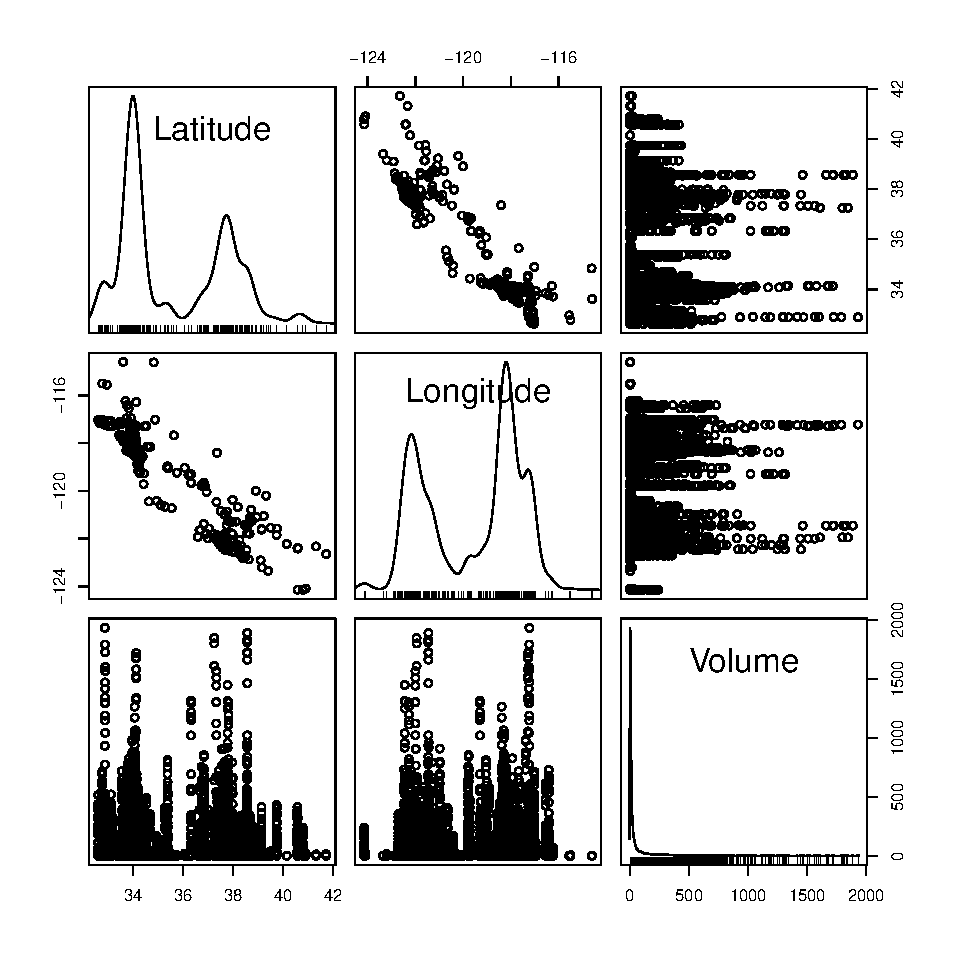
\includegraphics[width=0.63\textwidth]{images/scatterPlot_v0.pdf}
        \end{center}
\end{frame}

\begin{frame}[allowframebreaks, fragile]
\frametitle{Scatterplot (v.1)}

To get a quick peak into the numerical variables and the trends in the data, modify arguments of \ttfamily scatterplotMatrix(): \normalfont
  		\begin{lstlisting}
?scatterplotMatrix # for documentation
library(car)		
data(quakes)
scatterplotMatrix(
	x = quakes[, 1:4], 
	reg.line = FALSE
	)
		\end{lstlisting}

        \begin{center}
         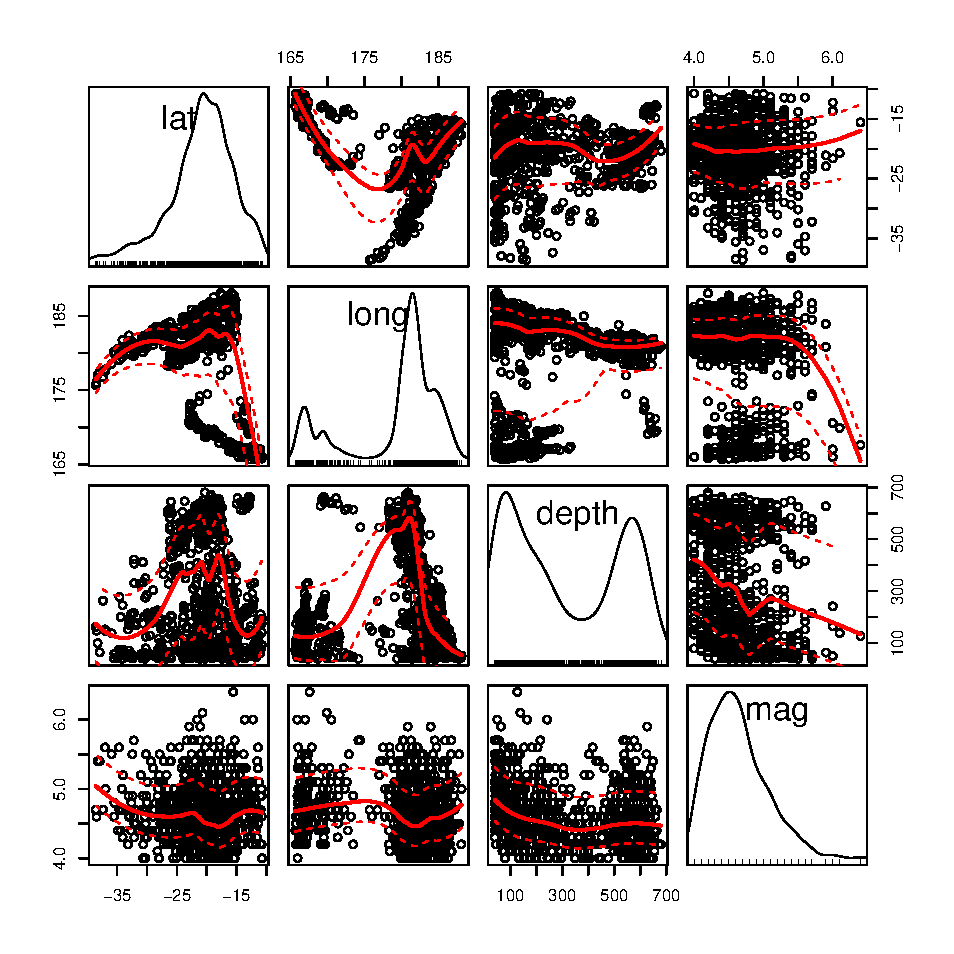
\includegraphics[width=0.63\textwidth]{images/scatterPlot_v1.pdf}
        \end{center}
\end{frame}


%%%%% New frame
\subsection{Histogram}
\begin{frame}[fragile, allowframebreaks]
\frametitle{'Nicer' Histogram (v0.1)}

To compare the frequencies of two variables side-by-side, use \ttfamily beanplot(): \normalfont

	\begin{lstlisting}
library(datasets)
library(beanplot)
data(ToothGrowth)
beanplot(
	len ~ supp, 
	data = ToothGrowth, 
	side = "both", 
	col = list( grey(0.5),grey(0.8) )
	)
	\end{lstlisting}

        \begin{center}
	         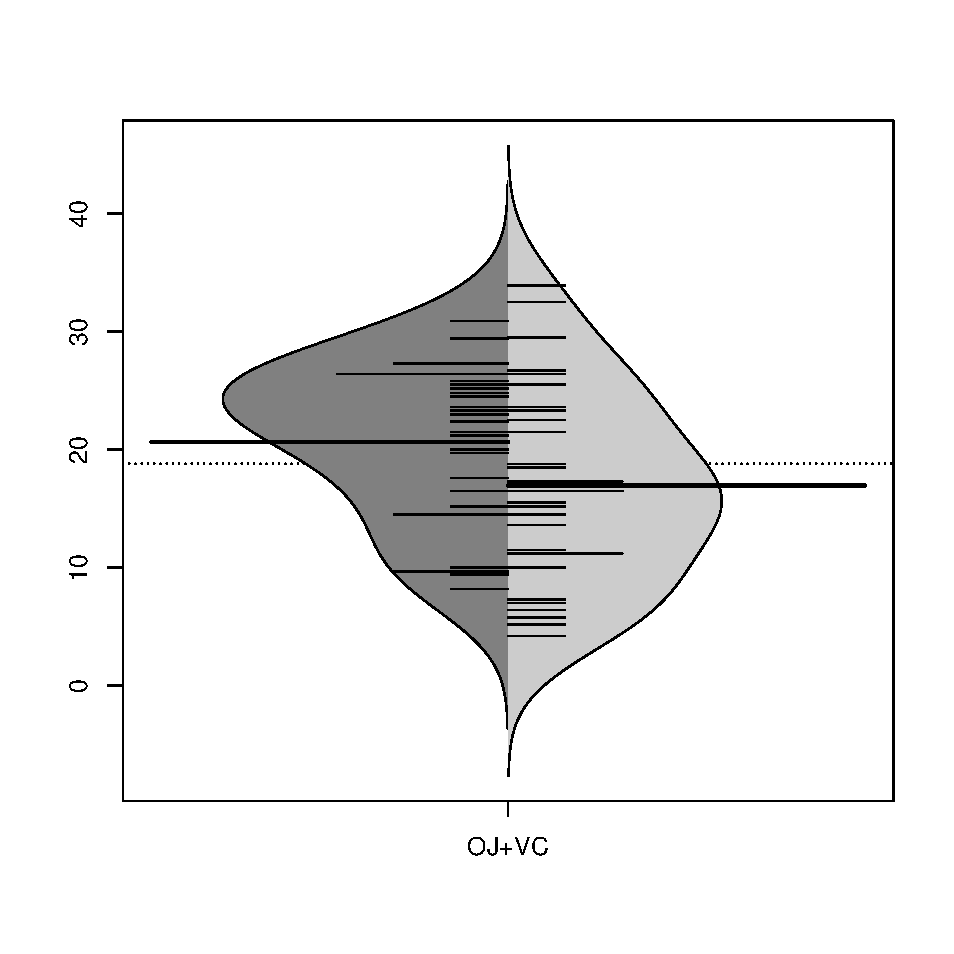
\includegraphics[width=0.65\textwidth]{images/beanplot_v0.pdf}
        \end{center}

\end{frame}

\begin{frame}[fragile, allowframebreaks]
\frametitle{'Nicer' Histogram (v0.2)}
To make the visual slightly more readable:

	\begin{lstlisting}[ basicstyle=\tiny ]
library(datasets)
library(beanplot)
data(ToothGrowth)
beanplot(
	len ~ supp, 
	data = ToothGrowth, 
	side = "both", 
	col = list( grey(0.5), c( grey(0.8),"white" )), 
	border = NA, 
	overallline = "median", 
	ll = 0.03
	)
legend(
	x = "bottomleft",
	fill=c( grey(0.5), grey(0.8) ), 
	legend=c( "Orange Juice", "Ascorbic Acid" )
	)
	\end{lstlisting}
	
        \begin{center}
	         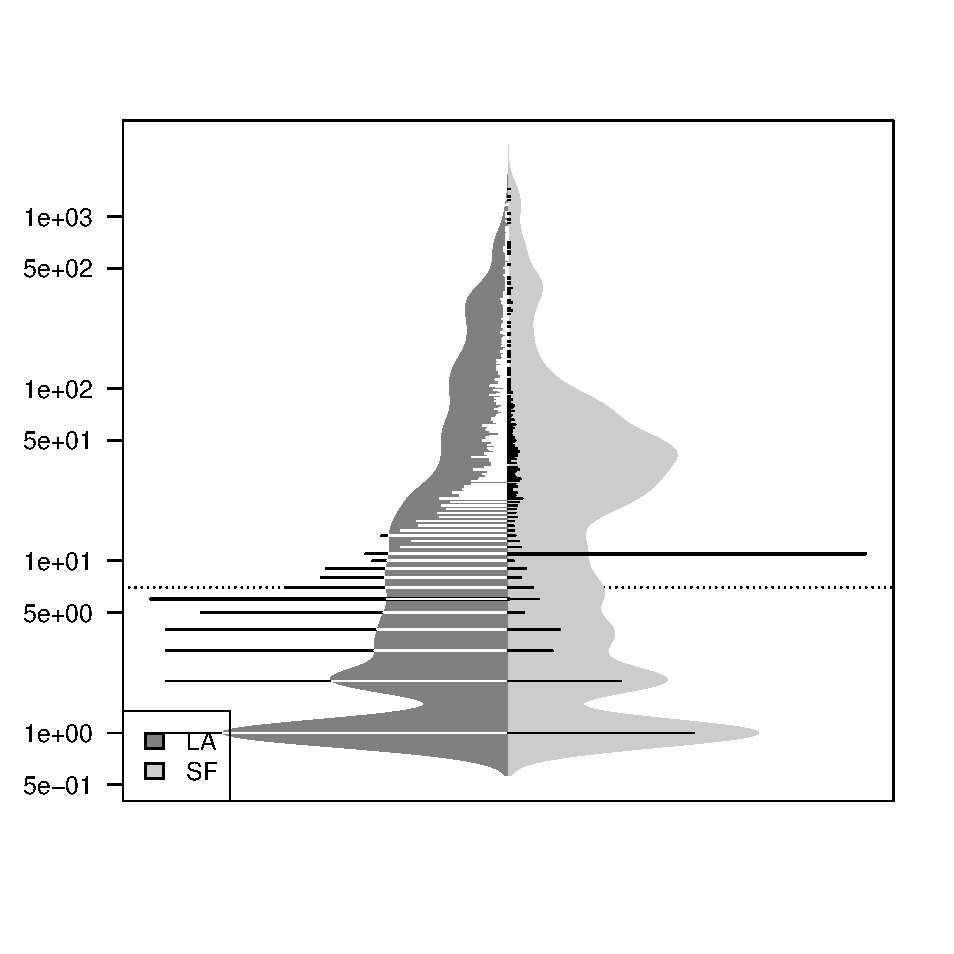
\includegraphics[width=0.65\textwidth]{images/beanplot.pdf}
        \end{center}
\end{frame}

%%% NOT WORK...
%
%library(lattice)
%split.screen(c(1,2))        # split display into two screens
%split.screen(c(2,1),2)      # split bottom half in two
%screen(1)                   # prepare screen 1 for output
%qqplot(ToothGrowth$len~ToothGrowth$supp)
%screen(4)                   # prepare screen 4 for output
% # boxplot(ToothGrowth$len~ToothGrowth$supp)
% beanplot(ToothGrowth$len~ToothGrowth$supp, col=list(grey(0.5),c(grey(0.8),"white")), border = NA, overallline = "median", ll=0.01, side="both")
%screen(1, FALSE)            # return to screen 1, but do not clear
%close.screen(all = TRUE)    # exit split-screen mode


%%%%%%%%%%%%%%%%%%%%%%%%%%%%%%%%%%%%%

% ------------------------------------------------------------
% ------------------------------------------------------------

% Exercise: compare distributions of Iris data
% ID outlier in dataset

\subsection{Exercise I}
\begin{frame}
	\frametitle{Exercise I}
	Compare the distributions of the sepal widths for the three species of irises (using the \ttfamily iris \normalfont data set).
\end{frame}